\documentclass{standalone}
\usepackage{tikz}
\usetikzlibrary{shapes.geometric, arrows.meta, positioning}

\tikzstyle{layer} = [rectangle, draw, minimum height=1cm, minimum width=2cm, align=center]
\tikzstyle{arrow} = [thick, -{Stealth}]

\begin{document}
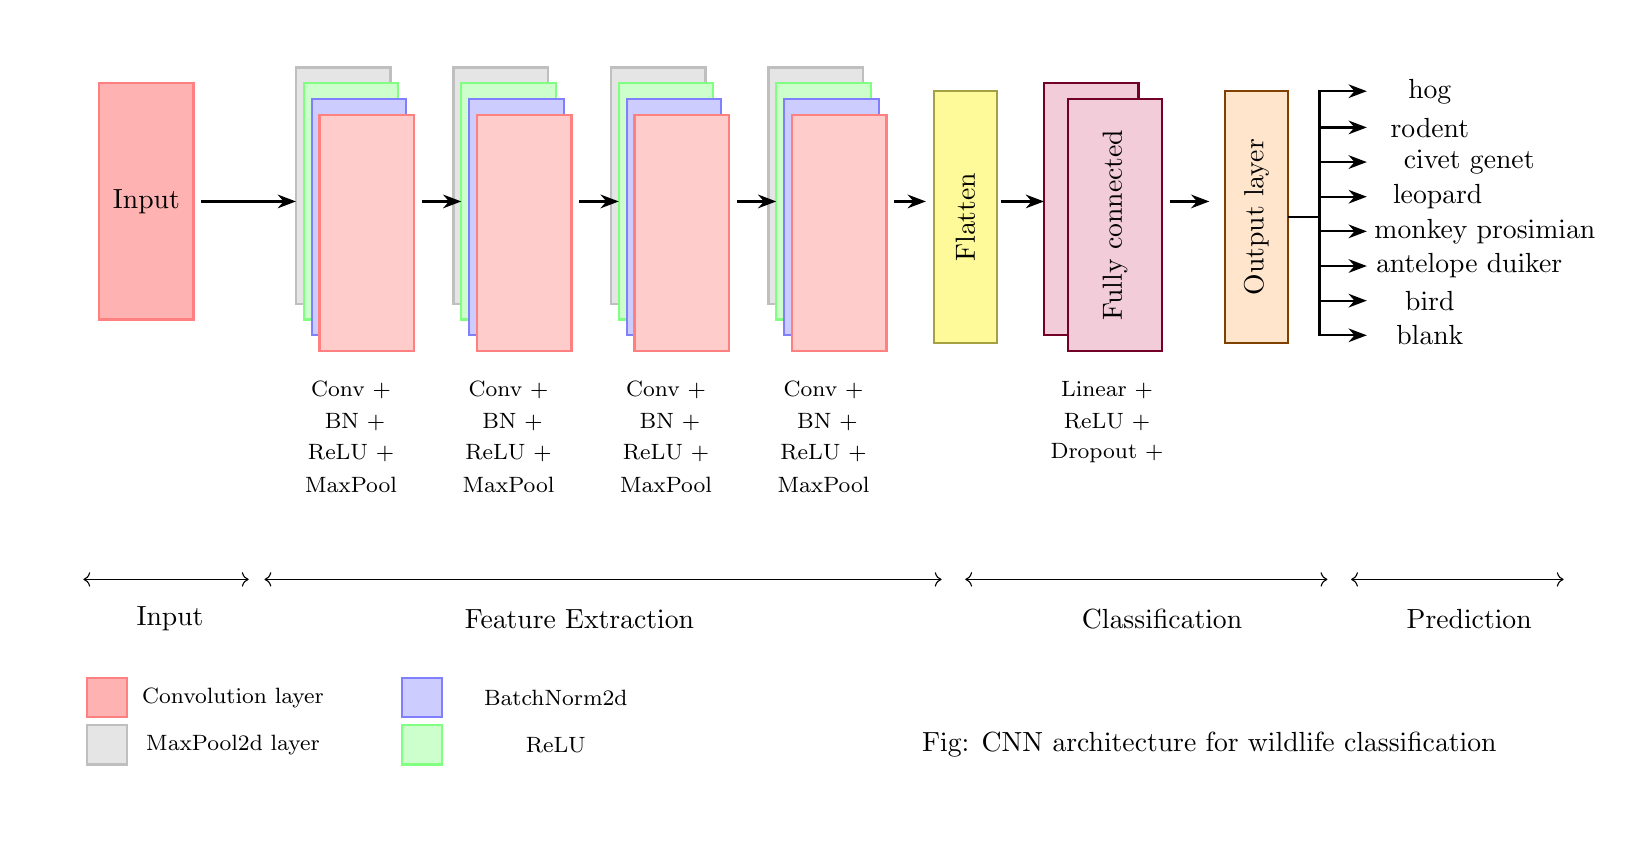
\begin{tikzpicture}[node distance=1.5cm and 1.5cm]
\draw[rectangle,draw=white](0,0)--(20,10);
\node[layer, fill=red!30, draw=red!50, minimum width=1.2cm,  minimum height=3cm, line width=.8pt,  align=center] (input) at (1.5,7.8) {Input};

\foreach \x in{4,6,8,10}{
     \node[ fill=gray!20, draw=gray!50, minimum width=1.2cm,  minimum height=3cm, line width=.8pt,  align=center] () at (\x,8) {};
}

\foreach \x in{4.10,6.10,8.10,10.10}{
     \node[fill=green!20, draw=green!50, minimum width=1.2cm,  minimum height=3cm, line width=.8pt,  align=center] () at (\x,7.8) {};
}
\foreach \x in{4.20,6.20,8.20,10.20}{
     \node[ fill=blue!20, draw=blue!50, minimum width=1.2cm,  minimum height=3cm, line width=.8pt,  align=center] () at (\x,7.6) {};
}
\foreach \x in{4.30,6.30,8.30,10.30}{
     \node[fill=red!20, draw=red!50, minimum width=1.2cm,  minimum height=3cm, line width=.8pt,  align=center] () at (\x,7.4) {};
}
% flatten layee 
\node[layer, fill=yellow!40, draw=yellow!60!black, minimum width=.8cm,  minimum height=3.2cm, line width=.8pt,  align=center] (flatten) at (11.9,7.6) {\rotatebox{90}{Flatten}};
% fully connected layer
\node[layer, fill=purple!20, draw=purple!60!black, minimum width=1.2cm,  minimum height=3.2cm, line width=.8pt,  align=center] (fc) at (13.5,7.7) {};
\node[layer, fill=purple!20, draw=purple!60!black, minimum width=1.2cm,  minimum height=3.2cm, line width=.8pt,  align=center] (fc) at (13.8,7.5) {\rotatebox{90}{Fully connected}};

% output layer                          
\node[layer, fill=orange!20, draw=orange!50!black, minimum width=.8cm,  minimum height=3.2cm, line width=.8pt,  align=center] (output) at (15.6,7.6) {\rotatebox{90}{Output layer}};
% arrows
\draw[arrow] (2.2,7.8) -- (3.4,7.8);
\draw[arrow] (5,7.8) -- (5.5,7.8);
\draw[arrow] (7,7.8) -- (7.5,7.8);
\draw[arrow] (9,7.8) -- (9.5,7.8);
\draw[arrow] (11,7.8) -- (11.4,7.8);
\draw[arrow] (12.35,7.8) -- (12.9,7.8);
\draw[arrow] (14.5,7.8) -- (15,7.8);
\draw[arrow] (16,7.6) -- (16.4,7.6)--(16.4,9.2)--(17,9.2);
\draw[arrow] (16,7.6) -- (16.4,7.6)--(16.4,6.1)--(17,6.1);;
\draw[arrow] (16.4,6.54)--(17,6.54);
\draw[arrow] (16.4,6.98)--(17,6.98);
\draw[arrow] (16.4,7.42)--(17,7.42);
\draw[arrow] (16.4,7.86)--(17,7.86);
\draw[arrow] (16.4,8.3)--(17,8.3);
\draw[arrow] (16.4,8.74)--(17,8.74);
%class names
\node at (17.8,9.2) {hog};
\node at (17.8,6.1) {blank};
\node at (17.8,6.54) {bird};
\node at (18.3,6.98) {antelope duiker};
\node at (18.5,7.42) {monkey prosimian};
\node at (17.9,7.86) {leopard};
\node at (18.3,8.3) {civet genet};
\node at (17.8,8.74) {rodent};

\foreach \x in{4.1,6.1,8.1,10.1}{
     \node at (\x,5.4) {\footnotesize{Conv $+$} };
}
\foreach \x in{4.1,6.1,8.1,10.1}{
     \node at (\x,5) { \footnotesize{ BN $+$} };
}
\foreach \x in{4.1,6.1,8.1,10.1}{
     \node at (\x,4.6) {\footnotesize{ReLU $+$} };
}
\foreach \x in{4.1,6.1,8.1,10.1}{
     \node at (\x,4.2) {\footnotesize{MaxPool}};
}
\draw[<->] (.7,3) -- (2.8,3);
\node[layer, fill=white, draw=white, minimum width=1cm,  minimum height=.5cm, line width=.8pt,  align=center] () at (1.8,2.5) {Input};
\draw[<->] (3,3) -- (11.6,3);
\node[layer, fill=white, draw=white, minimum width=1cm,  minimum height=.5cm, line width=.8pt,  align=center] () at (7,2.5) {Feature Extraction};
\draw[<->] (11.9,3) -- (16.5,3);
\node[layer, fill=white, draw=white, minimum width=1cm,  minimum height=.5cm, line width=.8pt,  align=center] () at (14.4,2.5) {Classification};
\draw[<->] (16.8,3) -- (19.5,3);
\node[layer, fill=white, draw=white, minimum width=1cm,  minimum height=.5cm, line width=.8pt,  align=center] () at (18.3,2.5) {Prediction};

\node at (13.7,5.4) {\footnotesize{Linear $+$} };
\node at (13.7,5) {\footnotesize{ReLU $+$} };
\node at (13.7,4.6) {\footnotesize{Dropout $+$} };

\node[layer, fill=red!30, draw=red!50,, minimum width=.5cm,  minimum height=.5cm, line width=.8pt,  align=center] () at (1,1.5) {};
\node at (2.6,1.5) {\footnotesize{Convolution layer} };
\node[layer, fill=gray!20, draw=gray!50, , minimum width=.5cm,  minimum height=.5cm, line width=.8pt,  align=center] () at (1,.9) {};
\node at (2.6,.9) {\footnotesize{MaxPool2d layer} };
\node[layer, fill=blue!20, draw=blue!50, minimum width=.5cm,  minimum height=.5cm, line width=.8pt,  align=center] () at (5,1.5) {};
\node at (6.7,1.5) {\footnotesize{BatchNorm2d} };
\node[layer,fill=green!20, draw=green!50, , minimum width=.5cm,  minimum height=.5cm, line width=.8pt,  align=center] () at (5,.9) {};
\node at (6.7,.9) {\footnotesize{ReLU} };

\node at (15,.9) {Fig: CNN architecture for wildlife classification};
\end{tikzpicture}

\end{document}
